\newpage

\section{Architettura}

\subsubsection{Informazioni generali}
\label{Architettura}
\begin{figure}[ht]
	\centering
	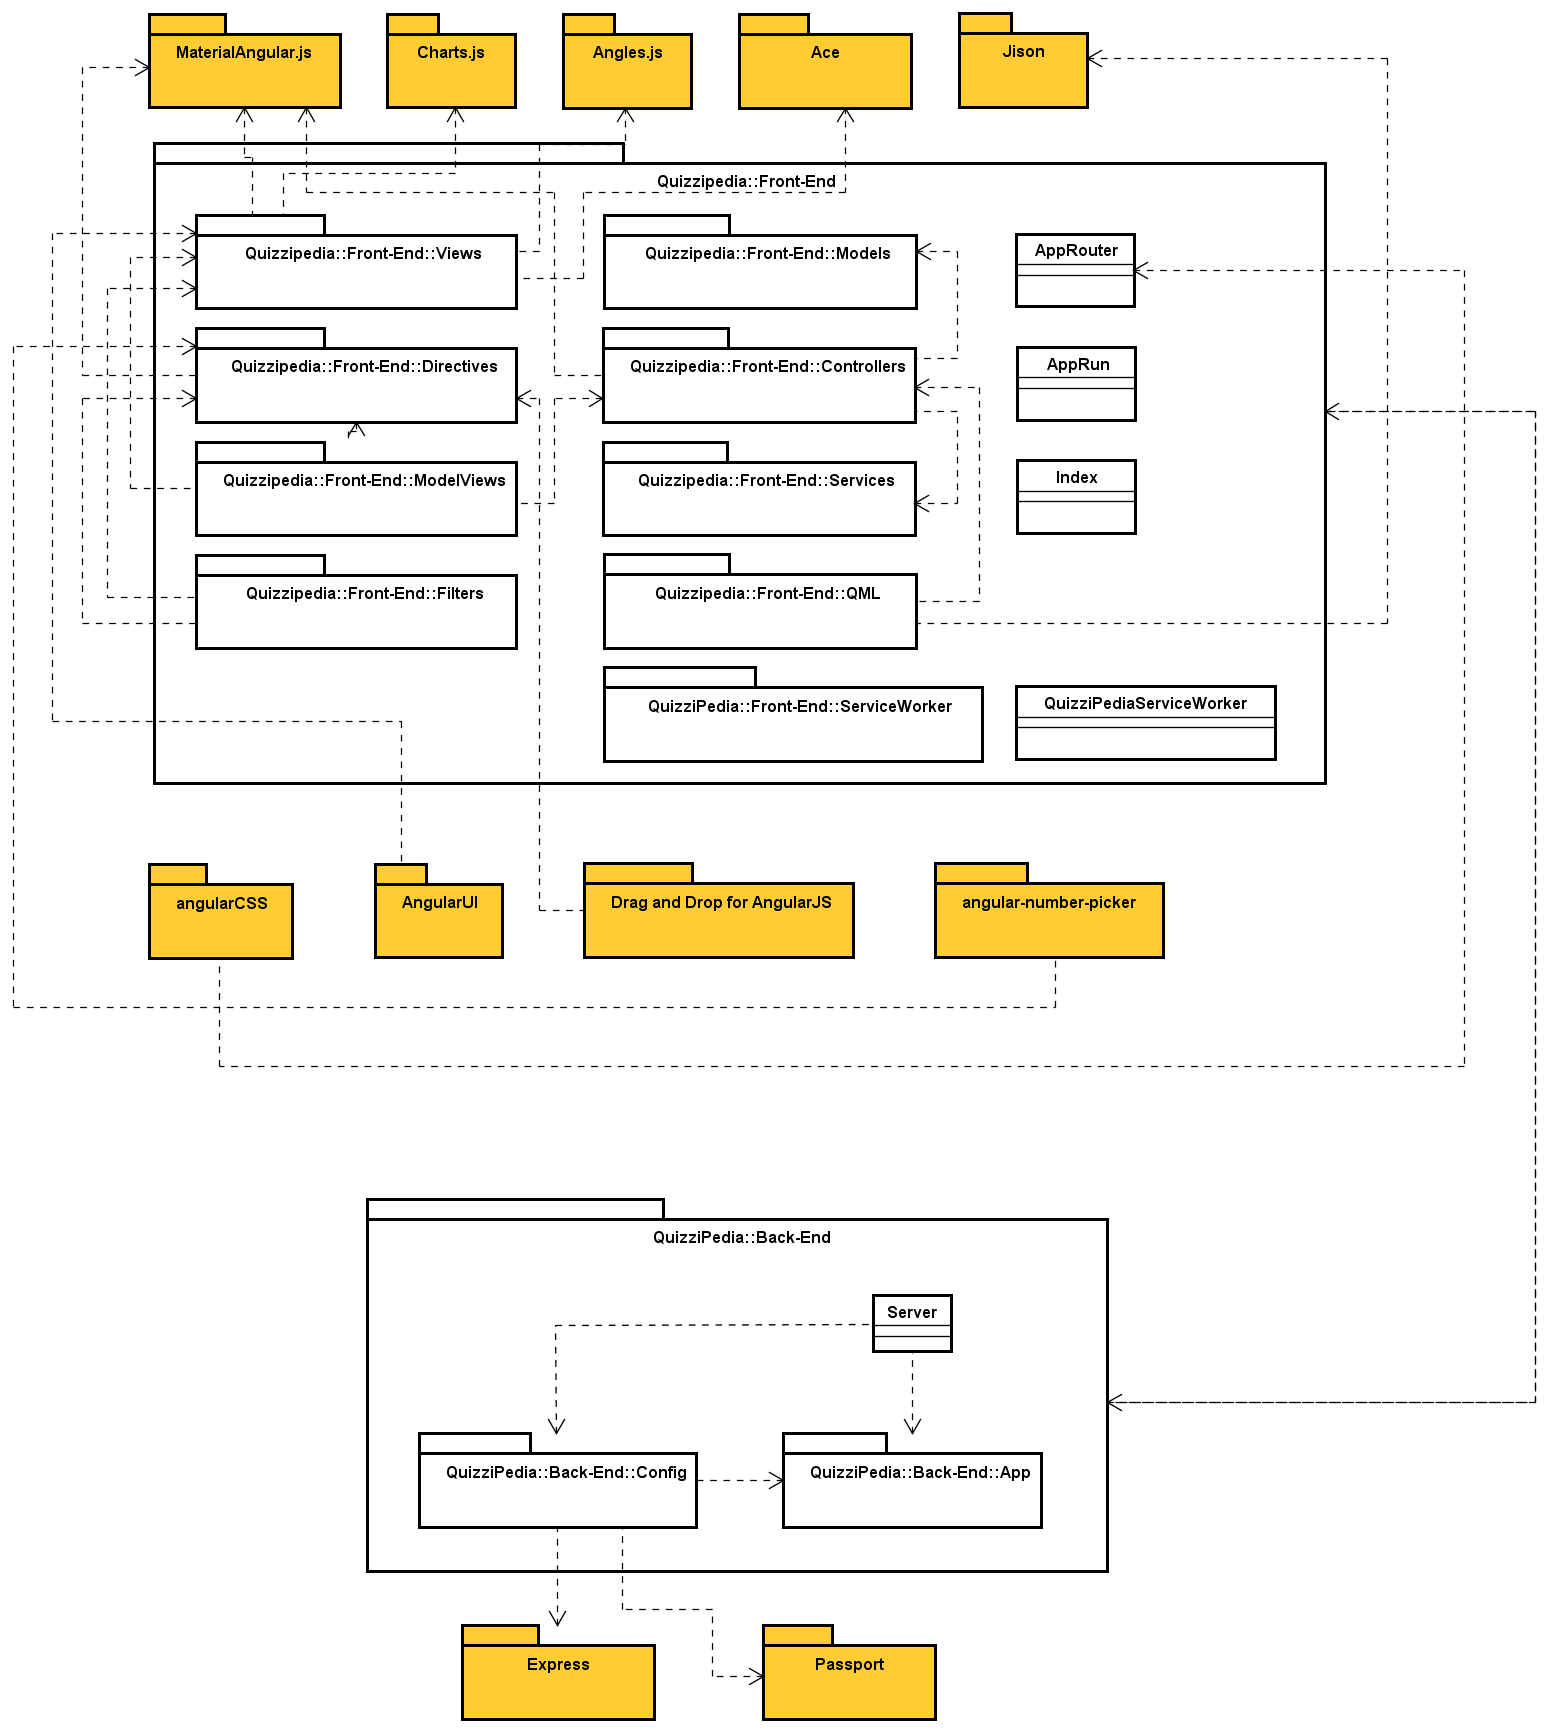
\includegraphics[scale=0.35]{UML/Package/QuizziPedia.png}
	\caption{Architettura}
\end{figure}
\FloatBarrier
\begin{itemize}
	\item \textbf{Descrizione}: architettura ad alto livello dell'applicazione \progetto;
	\item \textbf{Packages contenuti}:
	\begin{itemize}
		\item \texttt{QuizziPedia::Front-End}: \textit{package\ped{G}} contenente i \textit{packages\ped{G}} che compongono il Front-End;
		\item \texttt{QuizziPedia::Back-End}: \textit{package\ped{G}} contenente i \textit{packages\ped{G}} che compongono il Back-End;
		\item \texttt{MaterialAngular.js}: framework per lo sviluppo dei componenti grafici dell'applicazione;
		\item \texttt{Charts.js}: libreria per lo sviluppo dei grafici per la visualizzazione delle statistiche utente;
		\item \texttt{Angles.js}: libreria necessaria per integrare la libreria Charts.js all'interno dell'ambiente \textit{Angular\ped{G}};
		\item \texttt{TextAngular.js}: libreria per la creazione di un editor di testo all'interno delle pagine web per permettere all'utente di creare domande custom in linguaggio QML (si veda Appendice B);
		\item \texttt{Express}: framework Web di routing e middleware, con funzionalità sua propria minima: un’applicazione Express è essenzialmente una serie di chiamate a funzioni middleware.
	\end{itemize}
\end{itemize}
